% !TeX program = xelatex
\documentclass[12pt, a4paper]{article}
\usepackage{amsmath}
\usepackage{xeCJK}
\usepackage{amsmath}
\usepackage{amssymb}
\usepackage{parskip}
\usepackage{tikz}
\usepackage{enumitem}

\setmainfont{Latin Modern Roman}
\setCJKmainfont{Noto Serif CJK TC}

\title{Electrostatic field}

\begin{document}
\section*{Fundamental postulates of electrostatics in free space}
Electric field intensity of \textbf{E} \\
$\epsilon_0$: the permittivity of free space \\
\textbf{E} definition:
\begin{align*}
&\textbf{E} = \lim_{q \to 0} \frac{\textbf{F}}{q} \qquad (V/m) \\
& \vec{\textbf{F}} = q \vec{\textbf{E}}
\end{align*}
\\ \\
The fundamental postulates of electrostatics in free space. \\
\textbf{(\romannumeral1) The divergence of $\vec{E}$}
$$
\nabla \cdot \vec{E} = \frac{\rho_s}{\epsilon_0}
$$
$\rho_s$: the volume charge density of free charges $(C/m^2)$a 

\textbf{(\romannumeral2) The curl of $\vec{E}$}
$$
\nabla \times \vec{E} = 0
$$
Therefore,
$$
\int_{v} \nabla \cdot \vec{E} \text{d}v = \int_v \frac{\rho_s}{\epsilon_0} \text{d}v = \frac{1}{\epsilon_0} \int_v \rho_v \text{d}v
$$
By divergence theorem
$$
\oint_s \vec{E} \cdot \text{d}\vec{s} = \int_v \nabla \vec{E} \text{d}v = \frac{1}{\epsilon_0} \int_v \rho_v \text{d}v
$$
$\int_v \rho_v \text{d}v = Q$, total charge contained in volume $V$ bounded by surface $S$ \\
\textbf{Gauss's law}: the most important relations in elcectrostatices
$$
\oint_s \vec{E} \cdot \text{d} \vec{s} = \frac{Q}{\epsilon_0}
$$

For curl of $\vec{E}$
$$
\int_s \nabla \times \vec{E} \cdot \text{d} \vec{s} = 0
$$
By Sockes's theorem
$$
\int_s \nabla \vec{E} \cdot \text{d} \vec{s} = \oint_c \vec{E} \cdot \text{d} \vec{l} = 0
$$
\textbf{Kirchhoff's voltage law in circuit theory}: the alggebraic sum of volatge drops around any closed circuit is zero
\newpage
\section*{Coulomb's Law}



\tikzset{every picture/.style={line width=0.75pt}} %set default line width to 0.75pt        

\begin{tikzpicture}[x=0.75pt,y=0.75pt,yscale=-1,xscale=1]
%uncomment if require: \path (0,300); %set diagram left start at 0, and has height of 300

%Shape: Circle [id:dp8079472287983939] 
\draw  [dash pattern={on 4.5pt off 4.5pt}] (329.67,147.33) .. controls (329.67,105.91) and (363.25,72.33) .. (404.67,72.33) .. controls (446.09,72.33) and (479.67,105.91) .. (479.67,147.33) .. controls (479.67,188.75) and (446.09,222.33) .. (404.67,222.33) .. controls (363.25,222.33) and (329.67,188.75) .. (329.67,147.33) -- cycle ;
%Straight Lines [id:da6521053397492418] 
\draw    (349.71,167.34) -- (433.86,78.53) ;
%Straight Lines [id:da5830083394913639] 
\draw    (404.67,147.33) -- (410.9,133.28) -- (432.7,81.3) ;
\draw [shift={(433.86,78.53)}, rotate = 112.75] [fill={rgb, 255:red, 0; green, 0; blue, 0 }  ][line width=0.08]  [draw opacity=0] (5.36,-2.57) -- (0,0) -- (5.36,2.57) -- cycle    ;
%Shape: Circle [id:dp39356890481994955] 
\draw  [color={rgb, 255:red, 245; green, 166; blue, 35 }  ,draw opacity=1 ][fill={rgb, 255:red, 245; green, 166; blue, 35 }  ,fill opacity=1 ] (432.23,80.16) .. controls (432.23,79.26) and (432.96,78.53) .. (433.86,78.53) .. controls (434.76,78.53) and (435.49,79.26) .. (435.49,80.16) .. controls (435.49,81.06) and (434.76,81.79) .. (433.86,81.79) .. controls (432.96,81.79) and (432.23,81.06) .. (432.23,80.16) -- cycle ;
%Shape: Circle [id:dp05646441954953729] 
\draw  [dash pattern={on 4.5pt off 4.5pt}] (75,142) .. controls (75,100.58) and (108.58,67) .. (150,67) .. controls (191.42,67) and (225,100.58) .. (225,142) .. controls (225,183.42) and (191.42,217) .. (150,217) .. controls (108.58,217) and (75,183.42) .. (75,142) -- cycle ;
%Straight Lines [id:da8251753476788368] 
\draw  [dash pattern={on 4.5pt off 4.5pt}]  (150,142) -- (160.34,129.7) -- (198.87,84.99) ;
%Straight Lines [id:da1800558566319328] 
\draw    (150,142) -- (158.41,131.99) ;
\draw [shift={(160.34,129.7)}, rotate = 130.03] [fill={rgb, 255:red, 0; green, 0; blue, 0 }  ][line width=0.08]  [draw opacity=0] (5.36,-2.57) -- (0,0) -- (5.36,2.57) -- cycle    ;
%Straight Lines [id:da548849756727909] 
\draw [color={rgb, 255:red, 80; green, 227; blue, 194 }  ,draw opacity=1 ]   (198.87,84.99) -- (209.18,73.66) ;
\draw [shift={(211.2,71.44)}, rotate = 132.29] [fill={rgb, 255:red, 80; green, 227; blue, 194 }  ,fill opacity=1 ][line width=0.08]  [draw opacity=0] (5.36,-2.57) -- (0,0) -- (5.36,2.57) -- cycle    ;
%Shape: Circle [id:dp6758527607145025] 
\draw  [color={rgb, 255:red, 80; green, 227; blue, 194 }  ,draw opacity=1 ][fill={rgb, 255:red, 80; green, 227; blue, 194 }  ,fill opacity=1 ] (148.37,142) .. controls (148.37,141.1) and (149.1,140.37) .. (150,140.37) .. controls (150.9,140.37) and (151.63,141.1) .. (151.63,142) .. controls (151.63,142.9) and (150.9,143.63) .. (150,143.63) .. controls (149.1,143.63) and (148.37,142.9) .. (148.37,142) -- cycle ;
%Straight Lines [id:da8831564797966314] 
\draw    (349.71,167.34) -- (505.79,167.9) ;
\draw [shift={(507.79,167.91)}, rotate = 180.21] [color={rgb, 255:red, 0; green, 0; blue, 0 }  ][line width=0.75]    (10.93,-3.29) .. controls (6.95,-1.4) and (3.31,-0.3) .. (0,0) .. controls (3.31,0.3) and (6.95,1.4) .. (10.93,3.29)   ;
%Straight Lines [id:da9374690957139201] 
\draw    (349.71,167.34) -- (295.23,219.53) ;
\draw [shift={(293.79,220.91)}, rotate = 316.23] [color={rgb, 255:red, 0; green, 0; blue, 0 }  ][line width=0.75]    (10.93,-3.29) .. controls (6.95,-1.4) and (3.31,-0.3) .. (0,0) .. controls (3.31,0.3) and (6.95,1.4) .. (10.93,3.29)   ;
%Straight Lines [id:da18692547078781463] 
\draw    (349.71,167.34) -- (349.79,59.91) ;
\draw [shift={(349.79,57.91)}, rotate = 90.04] [color={rgb, 255:red, 0; green, 0; blue, 0 }  ][line width=0.75]    (10.93,-3.29) .. controls (6.95,-1.4) and (3.31,-0.3) .. (0,0) .. controls (3.31,0.3) and (6.95,1.4) .. (10.93,3.29)   ;
%Straight Lines [id:da37488071565462744] 
\draw    (404.67,147.33) -- (409.68,136.02) ;
\draw [shift={(410.9,133.28)}, rotate = 113.92] [fill={rgb, 255:red, 0; green, 0; blue, 0 }  ][line width=0.08]  [draw opacity=0] (5.36,-2.57) -- (0,0) -- (5.36,2.57) -- cycle    ;
%Straight Lines [id:da29998538014547405] 
\draw [color={rgb, 255:red, 80; green, 227; blue, 194 }  ,draw opacity=1 ]   (433.86,78.53) -- (439.26,64.83) ;
\draw [shift={(440.36,62.03)}, rotate = 111.5] [fill={rgb, 255:red, 80; green, 227; blue, 194 }  ,fill opacity=1 ][line width=0.08]  [draw opacity=0] (5.36,-2.57) -- (0,0) -- (5.36,2.57) -- cycle    ;
%Shape: Circle [id:dp8063979365413178] 
\draw  [color={rgb, 255:red, 80; green, 227; blue, 194 }  ,draw opacity=1 ][fill={rgb, 255:red, 80; green, 227; blue, 194 }  ,fill opacity=1 ] (403.04,147.33) .. controls (403.04,146.43) and (403.77,145.7) .. (404.67,145.7) .. controls (405.57,145.7) and (406.3,146.43) .. (406.3,147.33) .. controls (406.3,148.23) and (405.57,148.96) .. (404.67,148.96) .. controls (403.77,148.96) and (403.04,148.23) .. (403.04,147.33) -- cycle ;
%Straight Lines [id:da8159775669094996] 
\draw    (349.71,167.34) -- (401.85,148.36) ;
\draw [shift={(404.67,147.33)}, rotate = 160] [fill={rgb, 255:red, 0; green, 0; blue, 0 }  ][line width=0.08]  [draw opacity=0] (5.36,-2.57) -- (0,0) -- (5.36,2.57) -- cycle    ;

% Text Node
\draw (196.61,67.11) node [anchor=north west][inner sep=0.75pt]  [font=\footnotesize,color={rgb, 255:red, 80; green, 227; blue, 194 }  ,opacity=1 ]  {$E$};
% Text Node
\draw (166.11,99.61) node [anchor=north west][inner sep=0.75pt]  [font=\footnotesize]  {$R$};
% Text Node
\draw (158.61,134.44) node [anchor=north west][inner sep=0.75pt]  [font=\footnotesize]  {$\hat{a}_{R}$};
% Text Node
\draw (139.5,141.9) node [anchor=north west][inner sep=0.75pt]  [font=\footnotesize,color={rgb, 255:red, 80; green, 227; blue, 194 }  ,opacity=1 ]  {$q$};
% Text Node
\draw (424.94,55.94) node [anchor=north west][inner sep=0.75pt]  [font=\footnotesize,color={rgb, 255:red, 80; green, 227; blue, 194 }  ,opacity=1 ]  {$E$};
% Text Node
\draw (382.78,109.94) node [anchor=north west][inner sep=0.75pt]  [font=\footnotesize]  {$R$};
% Text Node
\draw (412.9,136.68) node [anchor=north west][inner sep=0.75pt]  [font=\footnotesize]  {$\hat{a}_{qP}$};
% Text Node
\draw (406.67,149.1) node [anchor=north west][inner sep=0.75pt]  [font=\footnotesize,color={rgb, 255:red, 80; green, 227; blue, 194 }  ,opacity=1 ]  {$q$};
% Text Node
\draw (384.53,155.73) node [anchor=north west][inner sep=0.75pt]  [font=\scriptsize]  {$R'$};
% Text Node
\draw (283.68,218.68) node [anchor=north west][inner sep=0.75pt]  [font=\small]  {$x$};
% Text Node
\draw (511.68,162.68) node [anchor=north west][inner sep=0.75pt]  [font=\small]  {$y$};
% Text Node
\draw (345.68,43.34) node [anchor=north west][inner sep=0.75pt]  [font=\small]  {$z$};
% Text Node
\draw (434.23,83.56) node [anchor=north west][inner sep=0.75pt]  [font=\footnotesize,color={rgb, 255:red, 245; green, 166; blue, 35 }  ,opacity=1 ]  {$P$};
\end{tikzpicture}


We know that $\vec{E} = \hat{a_R}E_R \quad$, $\text{d}\vec{s} = \hat{a_R} \text{d}s \quad$, $Q = q$
\begin{align*}
	&\oint_s \vec{E} \cdot \text{d} \vec{s} = \frac{Q}{\epsilon_0} \\
	&\oint_s (\hat{a_R}E_R) \cdot (\hat{a_R}\text{d}s) = \frac{q}{\epsilon_0} \\
	\because \quad &\hat{a_R} \cdot \hat{a_R} = 1 \\
	\Rightarrow \quad &E_R \oint_s \text{d}s = E_R(4 \pi R^2) = \frac{q}{\epsilon_0} \\
	\therefore \quad &E_R = \frac{q}{4 \pi \epsilon_0 R^2} \\
	&\vec{E} = \hat{a_R} \frac{q}{4 \pi \epsilon_0 R^2} \qquad (V/m)
\end{align*}
If $q$ is not at origin defined that \\
$\vec{R'}$: poistion vector of q, $\vec{R}$: position vector of a field point $P$ \\
$\hat{a_{qP}}$: unit vector from q to $P = \frac{\vec{R} - \vec{R'}}{\mid \vec{R} - \vec{R'} \mid}$ \\
$p = q_2, \quad \mid \vec{R_1} - \vec{R'} \mid: R_{12}, \quad \hat{a_{qP}}: \hat{a_{12}}$

\begin{align*}
	&\vec{E_P} = \hat{a_{12}} \frac{q_1}{4 \pi \epsilon_0 R_{12}^2} \\
	\because \quad&F_{12} = q_2 \vec{E_{12}} \\
	\therefore \quad&\text{a force } \vec{F_{12}} \text{ experienced by } q_2 \text { due to } E_{12} \text{ of } q_1 \text{ to } q_2 \\
	\therefore \quad &\vec{F_{12}} = q_2 \vec{E_{12}} = \hat{a_{12}} \frac{q_1 q_2}{4 \pi \epsilon_0 R_{12}^2} \qquad (N) \\
	&\text{This is Coulomb's law.}
\end{align*}
\newpage

\section*{Electric field due to a system of discrete charges}
n discrete point charges
$\Rightarrow$ electrostatic field $\propto \frac{\hat{a_R}q}{aR^2}$, superposition principle \\
$\therefore$ totla $\vec{E}$: vector sum
\begin{align*}
	\because \vec{E_p} &= \frac{q(\vec{R} - \vec{R'})}{4 \pi \epsilon_0 \mid R - R' \mid^3} \qquad (V/m) \\
	\therefore \vec{E} &= \frac{1}{4 \pi \epsilon_0} \left(\frac{q_1(\vec{R} - \vec{R_1'})}{\mid \vec{R} - \vec{R_1'} \mid^3} + \frac{q_2(\vec{R} - \vec{R_2'})}{\mid \vec{R} - \vec{R_2'} \mid^3} + ... + \frac{q_m(\vec{R} - \vec{R_m'})}{\mid \vec{R} - \vec{R_m'} \mid^3}\right) \\
	&= \frac{1}{4 \pi \epsilon_0} \sum_{k=1}^{n} \frac{q_m(\vec{R} - \vec{R'})}{\mid \vec{R} - \vec{R_k'} \mid^3}
\end{align*}

Electric field due to a system of continous distribution of a charge integrating (superposing)


\begin{center}
\tikzset{every picture/.style={line width=0.75pt}} %set default line width to 0.75pt        

\begin{tikzpicture}[x=0.75pt,y=0.75pt,yscale=-1,xscale=1]
%uncomment if require: \path (0,300); %set diagram left start at 0, and has height of 300

%Shape: Polygon Curved [id:ds5897513707362603] 
\draw   (140,61) .. controls (160,51) and (250,41) .. (230,61) .. controls (210,81) and (210,91) .. (230,121) .. controls (250,151) and (160,151) .. (140,121) .. controls (120,91) and (120,71) .. (140,61) -- cycle ;
%Shape: Cube [id:dp6766883267681462] 
\draw  [dash pattern={on 0.84pt off 2.51pt}] (156.19,80.58) -- (163.89,72.88) -- (181.88,72.88) -- (181.88,90.85) -- (174.17,98.56) -- (156.19,98.56) -- cycle ; \draw  [dash pattern={on 0.84pt off 2.51pt}] (181.88,72.88) -- (174.17,80.58) -- (156.19,80.58) ; \draw  [dash pattern={on 0.84pt off 2.51pt}] (174.17,80.58) -- (174.17,98.56) ;
%Shape: Circle [id:dp15163570923290592] 
\draw  [fill={rgb, 255:red, 0; green, 0; blue, 0 }  ,fill opacity=1 ] (166.59,87.72) .. controls (166.59,87.26) and (166.97,86.88) .. (167.43,86.88) .. controls (167.9,86.88) and (168.27,87.26) .. (168.27,87.72) .. controls (168.27,88.19) and (167.9,88.57) .. (167.43,88.57) .. controls (166.97,88.57) and (166.59,88.19) .. (166.59,87.72) -- cycle ;
%Curve Lines [id:da9178774861078874] 
\draw    (167.43,88.57) .. controls (152.58,69.67) and (158.81,48.93) .. (182.79,36.06) ;
\draw [shift={(184.27,35.28)}, rotate = 153.07] [color={rgb, 255:red, 0; green, 0; blue, 0 }  ][line width=0.75]    (6.56,-1.97) .. controls (4.17,-0.84) and (1.99,-0.18) .. (0,0) .. controls (1.99,0.18) and (4.17,0.84) .. (6.56,1.97)   ;
%Curve Lines [id:da4954648499836348] 
\draw    (230,121) .. controls (227.38,106.28) and (243.86,100.16) .. (257.92,94.03) ;
\draw [shift={(259.67,93.27)}, rotate = 156.04] [color={rgb, 255:red, 0; green, 0; blue, 0 }  ][line width=0.75]    (6.56,-1.97) .. controls (4.17,-0.84) and (1.99,-0.18) .. (0,0) .. controls (1.99,0.18) and (4.17,0.84) .. (6.56,1.97)   ;

% Text Node
\draw (186.99,26.16) node [anchor=north west][inner sep=0.75pt]  [font=\scriptsize]  {$\vec{R} \cdot P$};
% Text Node
\draw (268.78,93.54) node [anchor=north west][inner sep=0.75pt]  [font=\tiny] [align=left] {a continous charge distribution};
\end{tikzpicture}
\end{center}
The volume charge density $\rho_v \quad(C/m^3)$ differential element \\
$\Rightarrow$ like a point charge \\
The electric field intensity at field point $P$
\begin{align*}
	\text{d} \vec{E} &= \hat{a_R} \frac{\rho_v \text{d} v'}{4 \pi \epsilon_0 R^2} \\
	\vec{E} &= \frac{1}{4 \pi \epsilon_0} \int_{V'} \hat{a_R} \frac{\rho_v}{R^2} \text{d} v' \qquad(V/m)
\end{align*}
Surface charge density $\rho_s \quad(C/m^2)$\\
$$
\vec{E} = \frac{1}{4 \pi \epsilon_0} \int_{S'} \hat{a_R} \frac{\rho_s}{R^2} \text{d} s' \qquad (V/m)
$$
Line charge density $\rho_l \quad(C/m)$
$$
\vec{E} = \frac{1}{4 \pi \epsilon_0} \int_{L'} \hat{a_R} \frac{\rho_s}{R^2} \text{d} l' \qquad (V/m)
$$
\newpage

\section*{Gauss's law and applications}
$$
\oint_S \vec{E} \cdot \text{d} \vec{s} = \frac{Q}{\epsilon_0}
$$
$S$: any mathematical(hypothetical) closed surface(choosen for convenience) \\
\textbf{Gauss's law:} \\
\begin{enumerate}[label=\textcircled{\arabic*}]
	\item symmetry
	\item normal $\vec{E}$: constant
	\item easy, efficient
\end{enumerate}
suitable surface $\to$ Gaussian surface
\begin{center}


\tikzset{every picture/.style={line width=0.75pt}} %set default line width to 0.75pt        

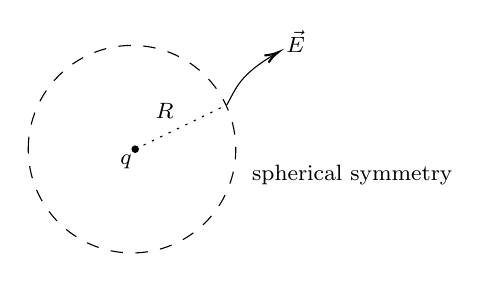
\begin{tikzpicture}[x=0.75pt,y=0.75pt,yscale=-1,xscale=1]
%uncomment if require: \path (0,300); %set diagram left start at 0, and has height of 300

%Shape: Circle [id:dp9514722883111292] 
\draw  [dash pattern={on 4.5pt off 4.5pt}] (176.67,122.67) .. controls (176.67,95.05) and (199.05,72.67) .. (226.67,72.67) .. controls (254.28,72.67) and (276.67,95.05) .. (276.67,122.67) .. controls (276.67,150.28) and (254.28,172.67) .. (226.67,172.67) .. controls (199.05,172.67) and (176.67,150.28) .. (176.67,122.67) -- cycle ;
%Shape: Circle [id:dp9613239940659304] 
\draw  [fill={rgb, 255:red, 0; green, 0; blue, 0 }  ,fill opacity=1 ] (226.67,122.67) .. controls (226.67,121.82) and (227.35,121.13) .. (228.2,121.13) .. controls (229.05,121.13) and (229.73,121.82) .. (229.73,122.67) .. controls (229.73,123.51) and (229.05,124.2) .. (228.2,124.2) .. controls (227.35,124.2) and (226.67,123.51) .. (226.67,122.67) -- cycle ;
%Straight Lines [id:da05670839945986905] 
\draw  [dash pattern={on 0.84pt off 2.51pt}]  (228.2,122.67) -- (272.35,101.36) ;
%Curve Lines [id:da45363422900130745] 
\draw    (272.35,101.36) .. controls (276.98,93.19) and (278.06,87.3) .. (295.46,76.92) ;
\draw [shift={(297.13,75.94)}, rotate = 149.93] [color={rgb, 255:red, 0; green, 0; blue, 0 }  ][line width=0.75]    (6.56,-1.97) .. controls (4.17,-0.84) and (1.99,-0.18) .. (0,0) .. controls (1.99,0.18) and (4.17,0.84) .. (6.56,1.97)   ;

% Text Node
\draw (236.8,99.4) node [anchor=north west][inner sep=0.75pt]  [font=\footnotesize]  {$R$};
% Text Node
\draw (219.8,124.4) node [anchor=north west][inner sep=0.75pt]  [font=\footnotesize]  {$q$};
% Text Node
\draw (299.8,64.4) node [anchor=north west][inner sep=0.75pt]  [font=\footnotesize]  {$\vec{E}$};
% Text Node
\draw (283.3,129) node [anchor=north west][inner sep=0.75pt]  [font=\footnotesize] [align=left] {spherical symmetry};
\end{tikzpicture}
\end{center}

\textbf{Exercise 3-6}
\begin{center}


\tikzset{every picture/.style={line width=0.75pt}} %set default line width to 0.75pt        

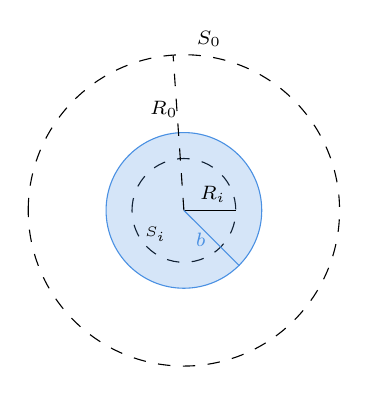
\begin{tikzpicture}[x=0.75pt,y=0.75pt,yscale=-1,xscale=1]
%uncomment if require: \path (0,300); %set diagram left start at 0, and has height of 300

%Shape: Circle [id:dp7948676111091696] 
\draw  [dash pattern={on 4.5pt off 4.5pt}] (245,147) .. controls (245,133.19) and (256.19,122) .. (270,122) .. controls (283.81,122) and (295,133.19) .. (295,147) .. controls (295,160.81) and (283.81,172) .. (270,172) .. controls (256.19,172) and (245,160.81) .. (245,147) -- cycle ;
%Shape: Circle [id:dp30976717903985285] 
\draw  [dash pattern={on 4.5pt off 4.5pt}] (195,147) .. controls (195,105.58) and (228.58,72) .. (270,72) .. controls (311.42,72) and (345,105.58) .. (345,147) .. controls (345,188.42) and (311.42,222) .. (270,222) .. controls (228.58,222) and (195,188.42) .. (195,147) -- cycle ;
%Shape: Circle [id:dp8903946301606492] 
\draw  [color={rgb, 255:red, 74; green, 144; blue, 226 }  ,draw opacity=1 ][fill={rgb, 255:red, 74; green, 144; blue, 226 }  ,fill opacity=0.23 ] (232.5,147) .. controls (232.5,126.29) and (249.29,109.5) .. (270,109.5) .. controls (290.71,109.5) and (307.5,126.29) .. (307.5,147) .. controls (307.5,167.71) and (290.71,184.5) .. (270,184.5) .. controls (249.29,184.5) and (232.5,167.71) .. (232.5,147) -- cycle ;
%Straight Lines [id:da9775377439203999] 
\draw    (270,147) -- (295,147) ;
%Straight Lines [id:da8707883506194768] 
\draw [color={rgb, 255:red, 74; green, 144; blue, 226 }  ,draw opacity=1 ]   (270,147) -- (296.8,173.7) ;
%Straight Lines [id:da8796239450352464] 
\draw  [dash pattern={on 4.5pt off 4.5pt}]  (270,147) -- (264.8,72.2) ;

% Text Node
\draw (250,153.9) node [anchor=north west][inner sep=0.75pt]  [font=\tiny,color={rgb, 255:red, 0; green, 0; blue, 0 }  ,opacity=1 ]  {$S_{i}$};
% Text Node
\draw (276.5,134.23) node [anchor=north west][inner sep=0.75pt]  [font=\scriptsize]  {$R_{i}$};
% Text Node
\draw (274.5,156.73) node [anchor=north west][inner sep=0.75pt]  [font=\scriptsize,color={rgb, 255:red, 74; green, 144; blue, 226 }  ,opacity=1 ]  {$b$};
% Text Node
\draw (252.5,93.23) node [anchor=north west][inner sep=0.75pt]  [font=\scriptsize]  {$R_{0}$};
% Text Node
\draw (275,59.23) node [anchor=north west][inner sep=0.75pt]  [font=\scriptsize]  {$S_{0}$};
\end{tikzpicture}
\end{center}
Give that \\
$\rho_v = -\rho_0 \qquad 0 \leq R \leq b$ \\
$\rho_v = 0 \quad  R > b$ \\
(where $\rho_0$ and $b$ is positive) \\
Find out $\vec{E} = ?$

\textbf{Sol.} \\
$\because$ source condition $\Rightarrow$ spherical symmetry \\
Guassian surface: concentric spherical surface \\
\newpage

\textbf{(a)} $0 \leq R \leq b$ \\
By Gauss's law:
$$
\oint_S \vec{E} \cdot \text{d} \vec{s} = \frac{Q}{\epsilon_0}
$$
Guassian surface: $S_i$ \\
$\vec{E}$ radial and constant magnitude
$$
\vec{E} = \hat{a_R} E_R
$$
$$
\text{d} \vec{s} = \hat{a_R} \text{d}s
$$
total outward $\vec{E}$ flux
\begin{align*}
	\oint_{S_i} \vec{E}\cdot \text{d} \vec{s} &= \oint_{S_i} \hat{a_R}E_R \cdot \hat{a_R}\text{d}s \\
  &= E_R \oint_{S_i} \text{d}s = 4 \pi R^2 E_R
\end{align*}
total charge
$$
Q = \int_V \rho_v \text{d}v = -\rho_0 \int_V \text{d}v = -\rho_0 \frac{4 \pi}{3} R^3
$$
From Gauss's law
\begin{align*}
	&4 \pi R^2 E_R = \rho_0 \frac{4 \pi}{3 \epsilon_0} R^3 \\
	&\Rightarrow E_R = \frac{-\rho_0R}{3 \epsilon_0} \\
	&\vec{E_R} = \hat{a_R} \frac{-\rho_0R}{3 \epsilon_0} \qquad 0 \leq R \leq b
\end{align*}

\textbf{(b)} $R \geq b$ \\
Guassian surface: $S_o$ \\
total outward $\vec{E}$ flux is same as above for $4 \pi R^2 E_R$ \\
total charge 
$$
Q = -\rho_0 \frac{4 \pi}{3} b^3
$$
Therefore
$$
\vec{E} = \hat{a_R} \frac{\rho_0b^3}{3 \epsilon_0 R^2} \qquad R \geq b
$$

\begin{center}
\tikzset{every picture/.style={line width=0.75pt}} %set default line width to 0.75pt        

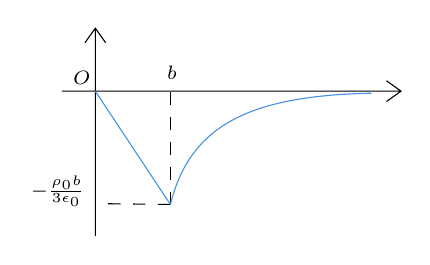
\begin{tikzpicture}[x=0.75pt,y=0.75pt,yscale=-1,xscale=1]
%uncomment if require: \path (0,300); %set diagram left start at 0, and has height of 300

%Shape: Axis 2D [id:dp9693784733434246] 
\draw  (56.31,94.32) -- (219.7,94.32)(72.43,64) -- (72.43,164) (212.7,89.32) -- (219.7,94.32) -- (212.7,99.32) (67.43,71) -- (72.43,64) -- (77.43,71)  ;
%Straight Lines [id:da23736978296751554] 
\draw [color={rgb, 255:red, 74; green, 144; blue, 226 }  ,draw opacity=1 ]   (72.43,94.32) -- (108.59,148.9) ;
%Straight Lines [id:da9057078320610283] 
\draw  [dash pattern={on 4.5pt off 4.5pt}]  (108.59,148.9) -- (108.59,93.7) ;
%Straight Lines [id:da12089306472761574] 
\draw  [dash pattern={on 4.5pt off 4.5pt}]  (108.59,148.9) -- (72.59,148.5) ;
%Curve Lines [id:da02692582189888093] 
\draw [color={rgb, 255:red, 74; green, 144; blue, 226 }  ,draw opacity=1 ]   (108.59,148.9) .. controls (118.19,110.1) and (147.79,96.5) .. (205.39,95.3) ;

% Text Node
\draw (105.7,81.17) node [anchor=north west][inner sep=0.75pt]  [font=\scriptsize]  {$b$};
% Text Node
\draw (40.1,133.97) node [anchor=north west][inner sep=0.75pt]  [font=\scriptsize]  {$-\frac{\rho _{0} b}{3\epsilon _{0}}$};
% Text Node
\draw (60.5,83.37) node [anchor=north west][inner sep=0.75pt]  [font=\scriptsize]  {$O$};
\end{tikzpicture}
\end{center}

\end{document}
